\documentclass{article}
\usepackage{graphicx,spconf,amsmath,amssymb,subfigure,color,hyperref}
\definecolor{darkgreen}{rgb}{0,0.5,0}
\newcommand{\Ntrg}{\big[N_{p=1, m=1} + \lambda \big] + \big[N_{p=1, m=2} + \lambda \big] + \ldots + \big[N_{p=1, m=M} + \lambda \big]}
\newcommand{\jointcnt}{\sum\limits_{n_{trg}=1}^{N_{trg}}I(X_p=x_p, X_{P-1}=x_{P-1})}
\newcommand{\singlecnt}{\sum\limits_{n_{trg}=1}^{N_{trg}}I(X_{P-1}=x_{P-1})}
\newcommand{\singlep}{p(X_{P-1}=x_{P-1})}
\newcommand{\singlepone}{p(X_{P-1}=1)}
\newcommand{\singleptwo}{p(X_{P-1}=2)}
\newcommand{\singlepM}{p(X_{P-1}=M)}
\newcommand{\condp}{p(X_p=x_p | X_{P-1}=x_{P-1})}
\newcommand{\jointp}{p(X_p=x_p, X_{P-1}=x_{P-1})}
\newcommand{\KmeansOuterSum}{\sum\limits_{k=1}^K}
\newcommand{\KmeansInnerSum}{\sum\limits_{{i=1 \atop x_i \in \mathcal{C}_k}}^N}
\newcommand{\KmeansSum}{\KmeansOuterSum \KmeansInnerSum}
\newcommand{\RVQInnerSum}{\sum\limits_{{i=1 \atop g_i \mapsto m_{\rho, s}}}^N}
\newcommand{\RVQOuterSum}{\sum_{m=1}^M}
\newcommand{\RVQsum}{\KmeansOuterSum \sum\limits_{{i=1 \atop g_i \in \mathcal{H}_k}}^N}
\newcommand{\KmeansInner}{{(x_i - y_k)}^2}
\newcommand{\RVQinner}{            {(x_i  - \hat{\mu}^{(k)})}^2}
\newcommand{\RVQinneralternate}{{(g_i - \mu_\rho^{(k)})}^2}
\newcommand{\RVQinneralternatealternate}{{(g_i - m_{\rho, s})}^2}
\newcommand{\KmeansError}{\KmeansSum \KmeansInner}
\newcommand{\RVQerror}     {\KmeansSum \RVQinner}
\newcommand{\RVQerroralternate}{\RVQsum \RVQinneralternate}
\newcommand{\RVQunit}{x_i -\bigg(\sum_{p=1}^P\mu^{(k)}_p\bigg)}
\newcommand{\RVQequivalentCodevector}{\sum_{p=1 }^P\mu^{(k)}_p}
\newcommand{\RVQequivalentCodevectorBroken}{\sum_{p=1 \atop p \neq \rho}^P\mu^{(k)}_p+ \mu^{(k)}_\rho}
\newcommand{\RVQmultipleKmeans}{x_i -\bigg(\RVQequivalentCodevectorBroken\bigg)}
\newcommand{\RVQmultipleKmeansone}{x_i -\bigg(\sum_{p=2}^P\mu^{(k)}_p+ \mu^{(k)}_\rho\bigg)}
\newcommand{\RVQmultipleKmeansonealternate}{\bigg(x_i -\sum_{p=1 \atop p \neq \rho}^P\mu^{(k)}_p\bigg) - \mu^{(k)}_\rho}
\newcommand{\RVQmultipleKmeanstwo}{x_i -\bigg(\sum_{p=1 \atop p \neq 2}^P\mu^{(k)}_p+ \mu^{(k)}_\rho\bigg)}
\newcommand{\RVQmultipleKmeansT}{x_i -\bigg(\sum_{p=1}^{P-1}\mu^{(k)}_p+ \mu^{(k)}_\rho\bigg)}
\newcommand{\EucMatrix}
{
\left[
\begin{array}{lll}
r_{11} & r_{12} & t_x \\ 
r_{21} & r_{22} & t_y \\ 
0 & 0 & 1 \\ 
\end{array}
\right]
}	

\newcommand{\SimMatrix}
{
\left[
\begin{array}{lll}
sr_{11} & sr_{12} & t_x \\ 
sr_{21} & sr_{22} & t_y \\
0 & 0 & 1 \\ 
\end{array}
\right]
}

\newcommand{\AffMatrix}
{
\left[
\begin{array}{lll}
a &b & t_x \\ 
c & d & t_y \\
0 & 0 & 1 \\
\end{array}
\right]
}

\newcommand{\ProjMatrix}
{
\left[
\begin{array}{lll}
h_{11} & h_{12} & h_{13} \\ 
h_{21} & h_{22} & h_{23} \\ 
h_{31} & h_{32} & h_{33} \\ 
\end{array}
\right]
}

\newcommand{\RotMatrixTheta}
{
\left[
\begin{array}{rr}
\cos(\theta) & -\sin(\theta) \\ 
\sin(\theta) & \cos(\theta) \\ 
\end{array}
\right]
}

\newcommand{\RotMatrixPhi}
{
\left[
\begin{array}{rr}
\cos(\phi) & -\sin(\phi) \\ 
\sin(\phi) & \cos(\phi) \\ 
\end{array}
\right]
}

\newcommand{\RotMatrixminusPhi}
{
\left[
\begin{array}{rr}
\cos(-\phi) & -\sin(-\phi) \\ 
\sin(-\phi) & \cos(-\phi) \\ 
\end{array}
\right]
}


\newcommand{\EigenvalueMatrix}
{
\left[
\begin{array}{cc}
\lambda_1 & 0\\
0 & \lambda_2
\end{array}
\right]
}

\newcommand{\bigMatrix}
{
s \left[
\begin{array}{cc}
 (r)(a) + b &  (r)(d) - c \\
 (r)(c) - d &  (r)(b) + a
\end{array}
\right]
}


\newcommand{\bigMatrixTwo}
{
\left[
\begin{array}{cc}
(\lambda_2) p + (\lambda_1) q & (\lambda_2) s  - (\lambda_1) r \\
(\lambda_2) r  - (\lambda_1) s & (\lambda_2) q + (\lambda_1) p
\end{array}
\right]
}
\newcommand{\dr}{(\mathbf{x}_i-\boldsymbol\mu_k)^T(\mathbf{x}_i-\boldsymbol\mu_k) + \lambda({P_{\textrm{max}}-P_i})}

\title{MODELING OF SMALL-SCALE HELICOPTER DYNAMICS USING RESIDUAL VECTOR QUANTIZATION IN A MACHINE LEARNING FRAMEWORK}
\name{Salman Aslam}
\address{National University of Sciences and Technology, Islamabad, Pakistan\\salman@gatech.edu}	
\begin{document}
\ninept
\maketitle
\begin{abstract}
In this paper, we present the first step towards modeling the dynamics of a small-scale helicopter using Residual Vector Quantization (RVQ).  Vector quantization (VQ) is frequently used in the Communications and Signal Processing literature.  A type of VQ called Residual Vector Quantization (RVQ) has received less attention, primarily due to the difficulty in generating stable designs.  To the best of our knowledge, this work is the first application of RVQ in a Machine Learning framework to understand helicopter dynamics.  Our initial investigation shows that RVQ can be used effectively to specify the dynamical state of a helicopter.  In future, we intend to expand this work and completely model helicopter dynamics using RVQ.
\end{abstract}

\begin{keywords}
Helicopter, vector quantization, Residual Vector Quantization, modeling
\end{keywords}

%--------------------------------------------------------------------------------------------------------------------------------------------------------------
\section{INTRODUCTION}
%--------------------------------------------------------------------------------------------------------------------------------------------------------------
%--------------------------------
\begin{figure}[h]
\centering	
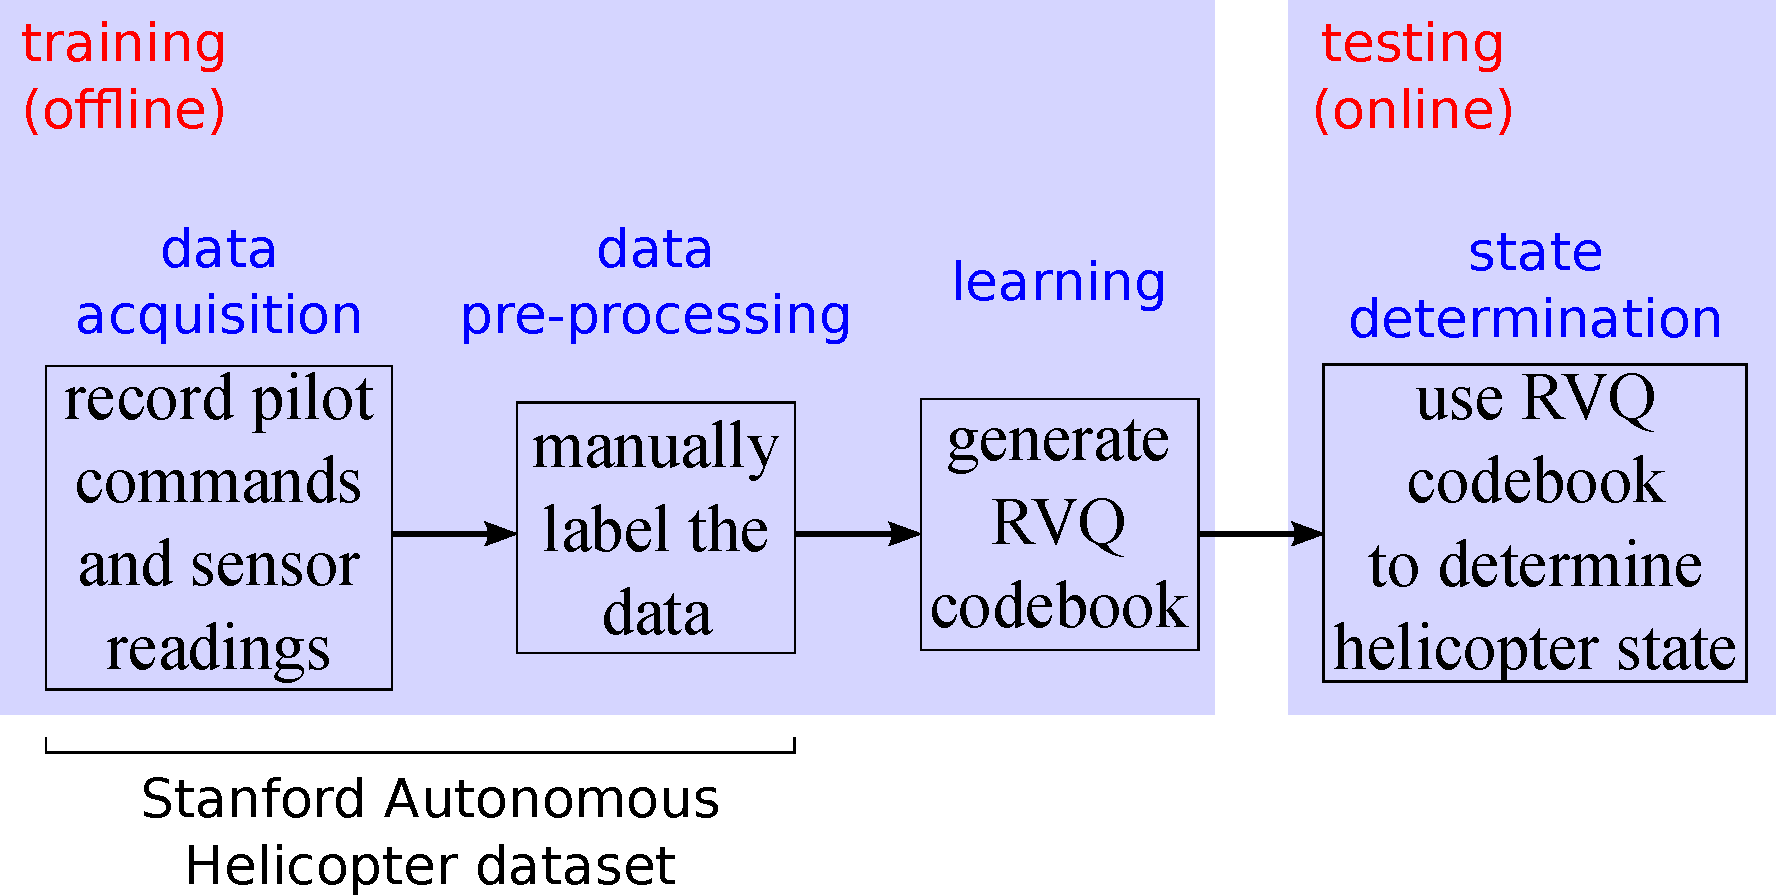
\includegraphics[width=0.5\textwidth]{figs/papers_ICAI2013_blockDiagram.pdf}
\caption{Block diagram of approach used in this paper.} 
\label{fig:blockDiagram}				
\end{figure}

A block diagram of our work is shown in Figure~\ref{fig:blockDiagram}.  We use data from the Stanford Helicopter dataset~\cite{dataset_StanfordHelicopter} to train RVQ codebooks for two different dynamical states of the helicopter.  This is done in an offline mode.  During run-time, the dynamical state of the helicopter is estimated using the RVQ codebook.



Small-scale helicopters, and in general, aerial robotics have received much attention in the past few years~\cite{2006_JNL_Heli_Wendel}.  This is due to their uses in security and surveillance applications, particularly those that require a hovering capability, search and rescue operations, industrial monitoring and inspection, remote telecast, urban planning and management, firefighting, power-line inspections, traffic monitoring, coastline monitoring, dam inspections and many more.  A helicopter with the 4 basic forces acting on it is shown in Figure~\ref{fig:heli_forces}.

%--------------------------------
\begin{figure}[t]
\centering	
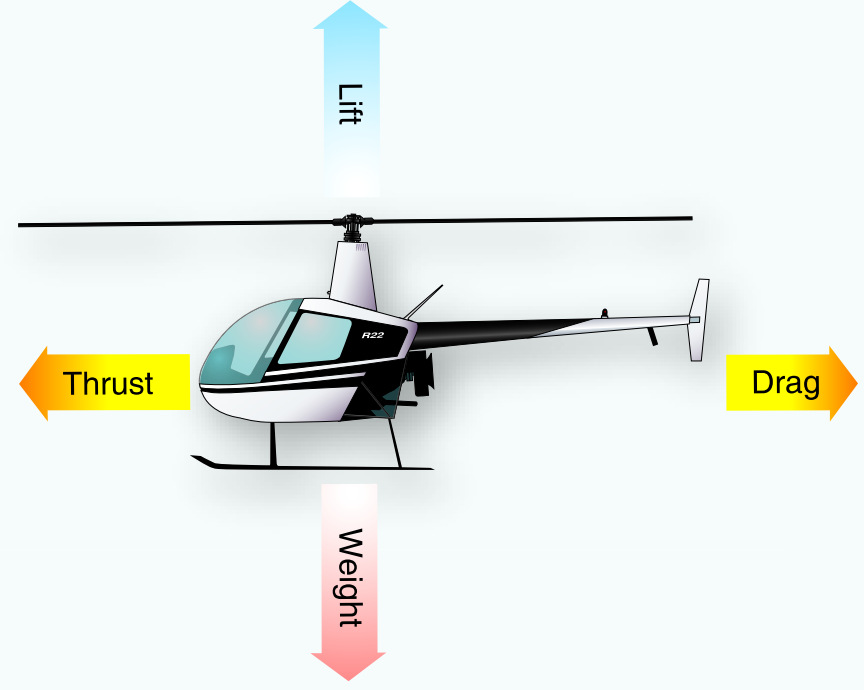
\includegraphics[width=0.35\textwidth]{figs/HELI_forces.png}
\caption{Helicopter and 4 basic forces acting on it~\cite{2012_BOOK_Heli_USDoT}.} 
\label{fig:heli_forces}				
\end{figure}


For an elastic body, such as a small scale helicopter, the general mathematical formulation of its flight, subject to aerodynamic (including propulsive) and gravitational forces through non-stationary air involves three set of equations: (a) The \emph{force equations}, which relate the motion of the mass-center to the external forces, (b) The \emph{moment equations}, which relate the rotation about the mass center to the external moments, and (c) The \emph{elastic equations} which relate the deformations of the structure to the loading imposed on it.  Likewise, the problems which have to be solved fall into three general categories: (a) \emph{Performance}, i.e., calculation of maximum speed, ceiling, range, etc., involve primarily the application of the force equations (b) \emph{Stability and control}, i.e., involve all three sets of equations but the moment equations are most important, and (c) \emph{Aeroelasticity} dominated primarily by the elastic equations~\cite{1959_BOOK_Flight_Etkin}. 

Given the complexity of this task, it is common to treat an aircraft as a rigid body.  The first formal derivation of the equations of motion for a rigid symmetric aircraft is usually attributed to Bryan (1911).  His treatment remains in use today with very few changes~\cite{2012_BOOK_Flight_Cook}.  It is usual to include aerodynamic descriptions in the equations of motion in the form of \emph{aerodynamic stability and control derivatives}.  Indeed, this is the approach pioneered by Bryan.  These derivatives can be estimated from flight test measurements using pattern recognition methods, such as multi-variable curve fitting.  This established and well developed experimental process results in coefficients in the aircraft state equation.  The derivatives can then be estimated from these coefficients (see Figure~\ref{fig:parameterID}).  


%--------------------------------
\begin{figure}[t]
\centering	
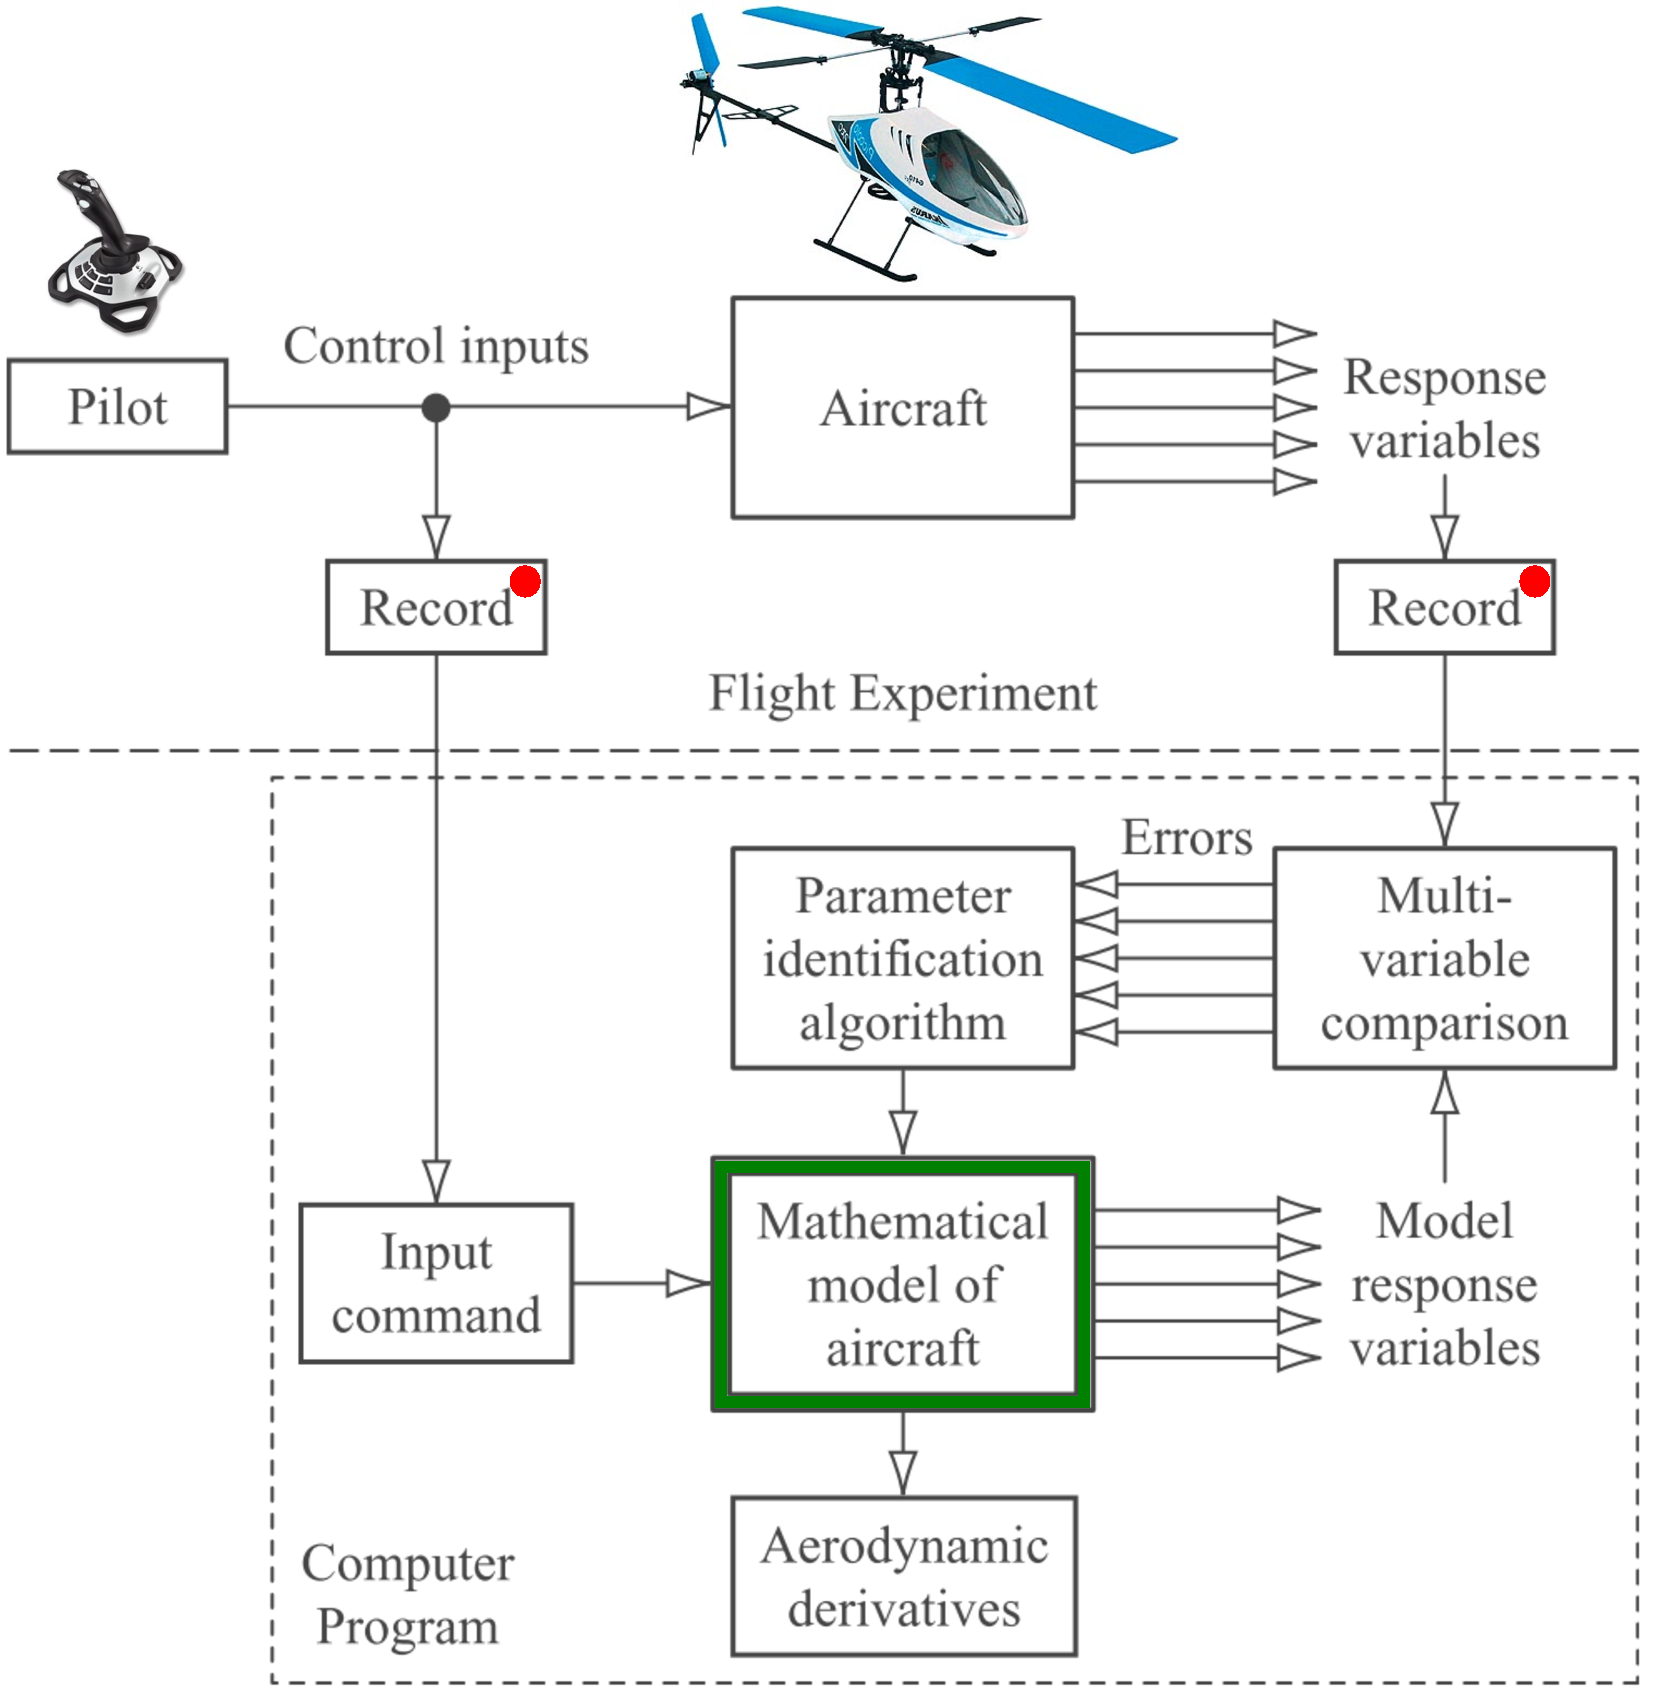
\includegraphics[width=0.5\textwidth]{figs/HELI_parameterID.pdf}
\caption{Parameter identification process~\cite{2012_BOOK_Flight_Cook}.} 
\label{fig:parameterID}				
\end{figure}

It may be noted that in helicopters, additional complexity is introduced by the rotating wing, i.e., the main and tail rotors, and associated flapping, feathering and lagging motions (Figure~\ref{fig:hinges}).  

%--------------------------------
\begin{figure}[h]
\centering
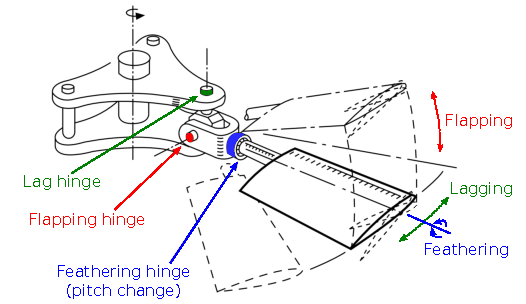
\includegraphics[width=0.5\textwidth]{figs/HELICOPTER_hinges.pdf}
\caption{Typical hinges on a helicopter~\cite{2001_BOOK_Heli_Bramwell}.}
\label{fig:hinges}
\end{figure}

A comparison of notation for forces, moments and linear and angular velocity components for a fixed-wing aircraft and helicopter is given in Figure~\ref{fig:notation}.  Next, we briefly introduce RVQ.

%--------------------------------
\begin{figure}[t]
\center
\subfigure[Commonly used notation for aircraft~\cite{1959_BOOK_Flight_Etkin}.]{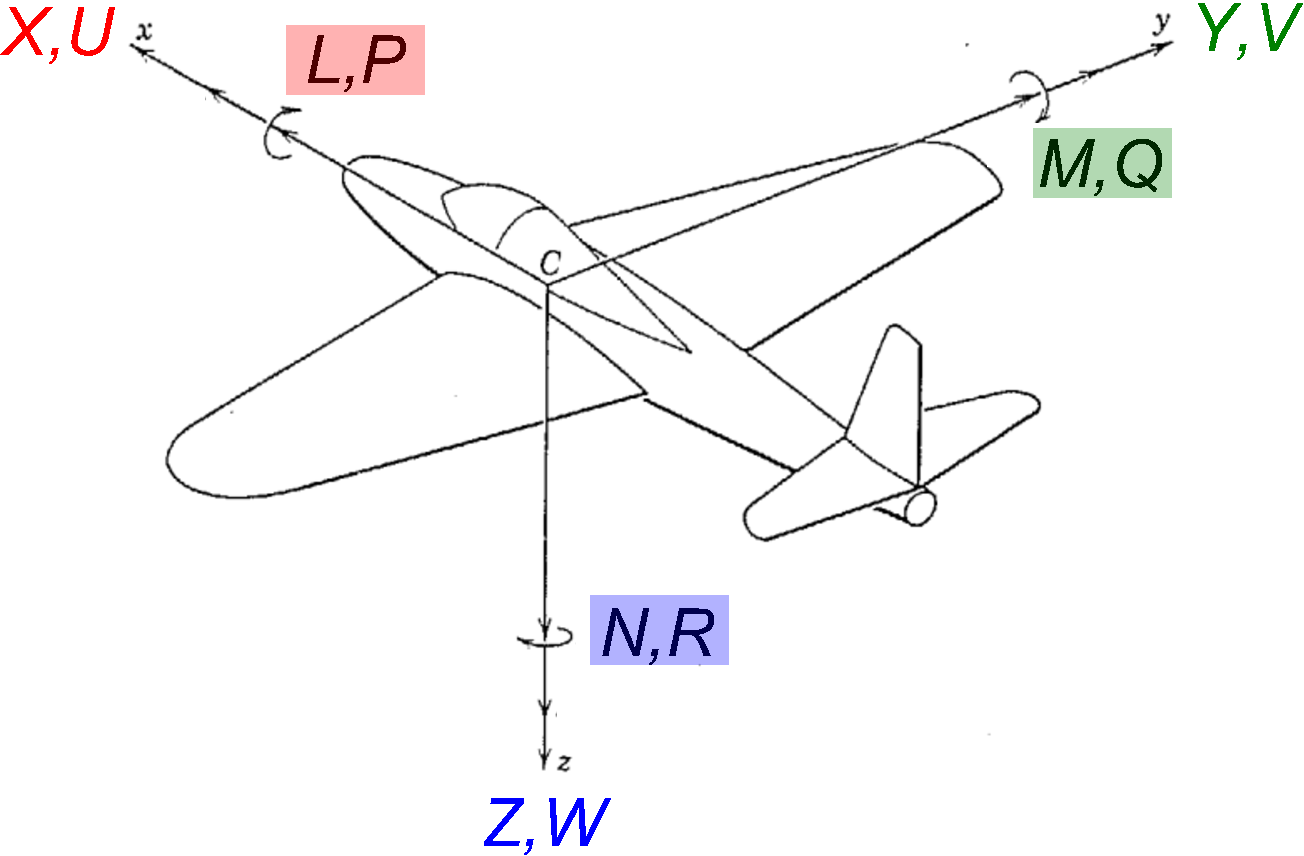
\includegraphics[width=0.4\textwidth]{figs/AIRCRAFT_notation.pdf}}
\hspace{0.5in}
\subfigure[Commonly used notation for helicopters~\cite{2011_BOOK_Heli_Raptis}.]{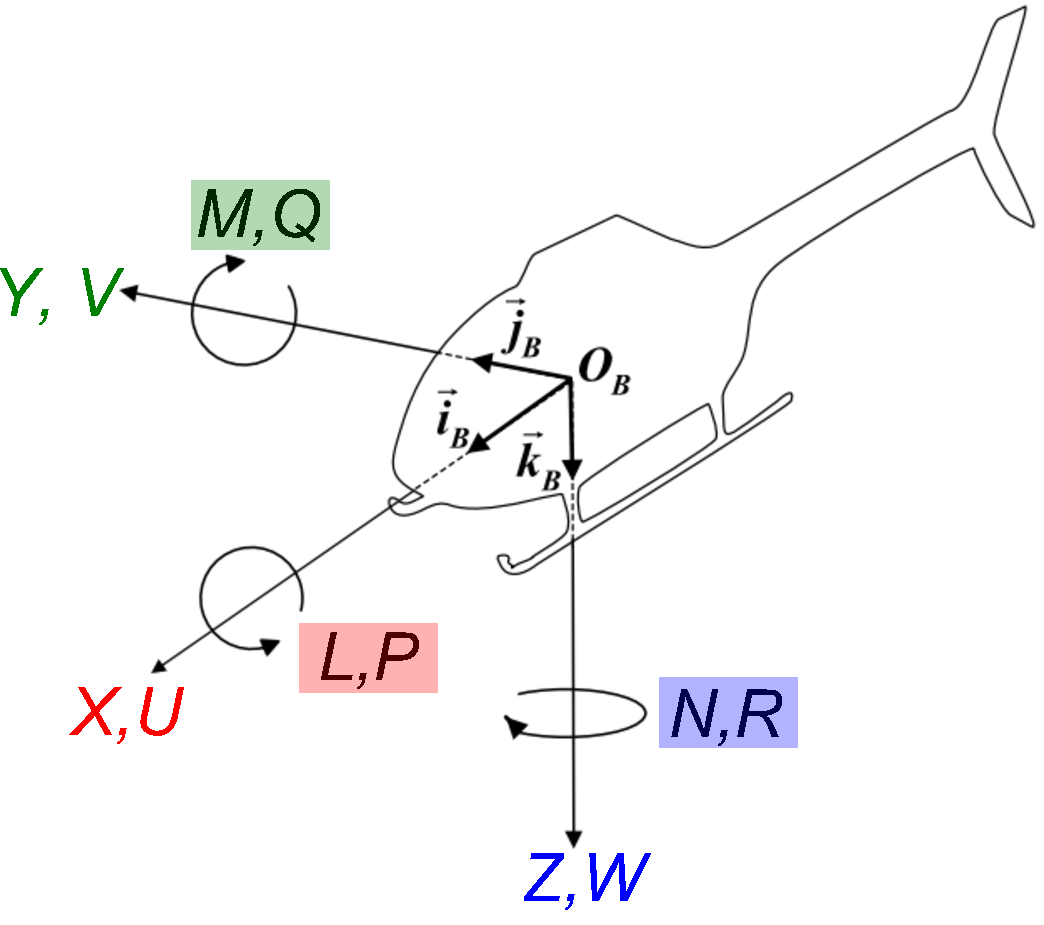
\includegraphics[width=0.32\textwidth]{figs/HELI_notation.pdf}}
\caption{Six aerodynamic forces and moments (rolling, pitching and yawing) acting on the aircraft are denoted by the triples [$X$,~$Y$,~$Z$] and [$L$,~$M$,~$N$] respectively (note that helicopters experience nine forces and moments due to three additional aileron, elevator and rudder hinge moments [$H_a$,~$H_e$,~$H_r$]).  The linear and angular velocity components are denoted by the triples [$U$,~$V$,~$W$] and [$P$,~$Q$,~$R$] respectively.  Note the standardized notation from very different time periods across different aircraft types and different authors.}   
\label{fig:notation}
\end{figure}




%The helicopter is a difficult and taxing aircraft to fly and generally requires autostabilization to restrict the pilot workload to a safe and comfortable level~\cite{2011_BOOK_Heli_Seddon}.
%
%Twelve non-linear differential equations are required to model the motion of an aircraft~\cite{1959_BOOK_Flight_Etkin}.  

%====================
\section{RVQ}
\label{sec:types_VQ}
%====================

%--------------------------------
\begin{figure}[t]
\centering	
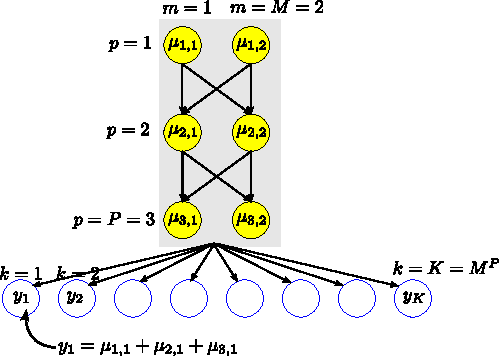
\includegraphics[width=0.5\textwidth]{figs/RVQ_trellis.pdf}
\caption{RVQ $\sigma$-tree, 3 stages, 2 code-vectors per stage, i.e., $P$=3, $M=2$.  This is a 3x2 $\sigma$-tree.} 
\label{fig:RVQ_sigma_tree}				
\end{figure}


Residual Vector Quantization, first introduced in 1982 by Juang~\cite{1982_CNF_SpeechRVQ_JuangGray} is a form of vector quantization (VQ).  Recall that the objective of VQ is to reduce output distortion and bring it close to the \emph{rate-distortion curve}.  A comprehensive analysis of the advantages of VQ, and therefore also of RVQ, over scalar quantization is explained in~\cite{1985_JNL_VQ_Makhoul} in three distinct areas: (a) axis rotation combined with scalar quantization, (b) arbitrary cell-shapes and (c) arbitrary code-vector placement.   However, in general, optimal placement of centroids (means) is not possible unless an exhaustive search is carried out over all code-vectors, as in structurally unconstrained \emph{Exhaustive Search Vector Quantizer} (ESVQ)~\cite{1996_JNL_AdvancesRVQ_Barnes}.  For a rate $r$ and dimension $D$, there are $K=2^{rD}$ code-vectors meaning that computational and memory cost are both exponential.  A solution is to constrain the VQ structure.  

One possible and widely used solution is to design a tree structured vector quantizer (TSVQ) as proposed in~\cite{1980_JNL_TSVQ_Buzo}.  A $P$-level binary TSVQ reduces the run-time search complexity to $\approx 2P$ but doubles the storage requirements~\cite{1996_JNL_AdvancesRVQ_Barnes}.    A method of reducing both run-time computational and storage complexity is to use a product code VQ~\cite{1991_BOOK_VQ_GershoGray}.  The idea is to partition a complex problem into numerous smaller problems.  Some examples include gain-shape VQ, mean-residual VQ, mean-gain-shape VQ and RVQ~\cite{1996_JNL_AdvancesRVQ_Barnes}.  

An RVQ trellis, also known as a $\sigma$-tree (sigma tree), is shown in Figure~\ref{fig:RVQ_sigma_tree}.  There are a total of $M$ columns indexed by $m$ and $P$ rows indexed by $p$.  Each row is also known as a \emph{stage}.  Each node of this tree, $\mu_{m,p}$ is called a \emph{stage code-vector} and is a centroid (mean) of a linear transformation of the data.  In Figure~\ref{fig:RVQ_sigma_tree}, there are 6 stage-code-vectors, 2 in each stage.  The leaf (terminal) nodes of this tree, also called \emph{equivalent code-vectors} or \emph{direct-sum codevectors} constitute what is known as the RVQ \emph{code-book}~\cite{2007_JNL_IDDM_Barnes}.  Each equivalent code-vector is created by summing a stage code-vector picked from each stage, and hence the term \emph{direct sum}.  There are $K=M^P$ possible unique direct sums or equivalent code-vectors.

The K-means objective function to be minimized for ESVQ, TSVQ and RVQ, for both the continuous and discrete cases, is the same.  For the discrete case, this function is given by,

\begin{equation}
e = \KmeansError
\label{Eqn:KmeansError}
\end{equation}

Here, there are $K$ classes and $N$ data points.  This minimization is commonly referred to as the GLA algorithm in the signal processing community.

If the partitions are known, then computing the optimal means (centroids) is a convex least squares optimization problem, otherwise it is an NP hard problem.

For RVQ, an equivalent code-vector, say the $k$-th equivalent code-vector, is created by simply summing together $P$ stage code-vectors.  This direct sum can be written as,

\begin{equation}
y_k = \mu_1^{(k)} + \mu_2^{(k)} + \ldots + \mu_P^{(k)}
\end{equation}

Substituting this in the distortion equation in Equation~\ref{Eqn:KmeansError} and grouping stage code-vectors so that the stage code-vector at the $\rho$-th stage remains separate gives us one equation per stage,
 
\begin{equation}
\begin{array}{llll}
e&= \KmeansSum{\bigg[\RVQmultipleKmeansone\bigg]}^2, \ \ \rho=1\\
&= \KmeansSum{\bigg[\RVQmultipleKmeanstwo\bigg]}^2, \ \ \rho=2\\
&\ \ \ \  \ \ \ \vdots\notag\\
&=\KmeansSum{\bigg[\RVQmultipleKmeansT\bigg]}^2, \ \ \rho=P 
\end{array}
\label{eqn:RVQ_Kmeans_2}
\end{equation}

Equation~\ref{eqn:RVQ_Kmeans_2} can be regrouped and written in compact notation as,

\begin{align}
e&= \KmeansSum{\bigg[\RVQmultipleKmeansonealternate\bigg]}^2, \ \ \rho=\{1, 2, \ldots P\}\notag\\
&={\RVQerroralternate}, \ \ \rho=\{1, 2, \ldots P\}
\label{eqn:RVQ_Kmeans_3}
\end{align}

where $g_i$ is called the \emph{graft residual}~\cite{1993_JNL_RVQDSC_Barnes} or the \emph{causal anti-causal (CAC) residual}~\cite{1993_JNL_RVQDSC_Barnes}.  This means that the RVQ objective function is now a coupled K-means problem.  In this coupled scenario, the design of each stage code-vector depends on stage code-vectors from all other stages, and not just prior stages.  This is the reasoning behind the causal anti-causal terminology.    Naturally, it is challenging to compute the centroids for one stage since this step changes the residual centroids for all other stages.  

%An RVQ is different from a traditional VQ in the sense that it partitions the input space $\mathbb{R}^D$ into $M$ cells.  The residual space, also in $\mathbb{R}^D$, is then partitioned again into $M$ cells.  This process is repeated $P$ times.  The advantage of this approach is that in obtaining $M^P$ partitions, we need to run our partitioning algorithm $P$ times and generate $M$ partitions at each stage.  In traditional VQ, the partitioning algorithm would run once but have to create $M^P$ partitions.  For the binary case (two code-vectors per stage, $M=2$) and a total of 8 stages ($P$=8), RVQ only requires 16 searches.  In $ESVQ$, this would require 256.  Therefore, exponential complexity is reduced to linear complexity.  In general, structurally constrained quantizers such as RVQ cannot provide performance as good as ESVQ.  However, since they are able to more efficiently implement codes, larger and larger vector sizes can be used, and if carefully designed, can achieve better performance that ESVQ for a given computational cost~\cite{1996_JNL_AdvancesRVQ_Barnes}.

%====================
\section{EXPERIMENTS}
%====================

%--------------------------------
\begin{figure}[t]
\centering	
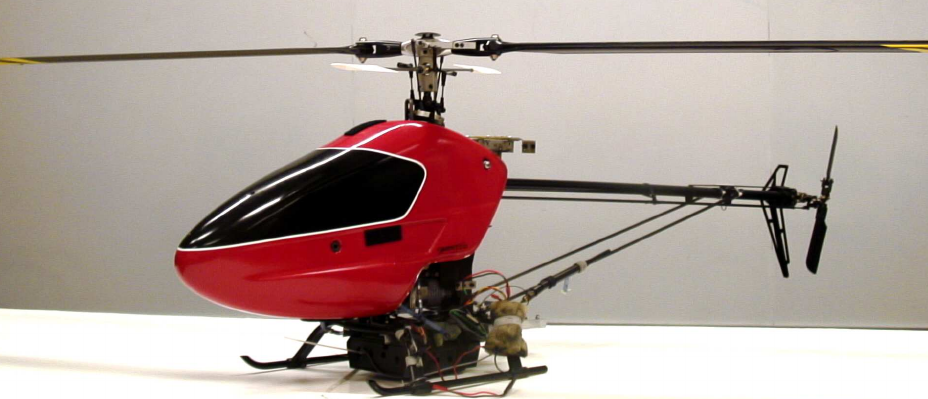
\includegraphics[width=0.45\textwidth]{figs/papers_ICAI2013_heli.png}
\caption{The Xcell Tempest helicopter used in the Stanford helicopter dataset~\cite{dataset_StanfordHelicopter}.} 
\label{fig:heli}				
\end{figure}

%%%%\begin{figure*}[t]
%%%%\centering	
%%%%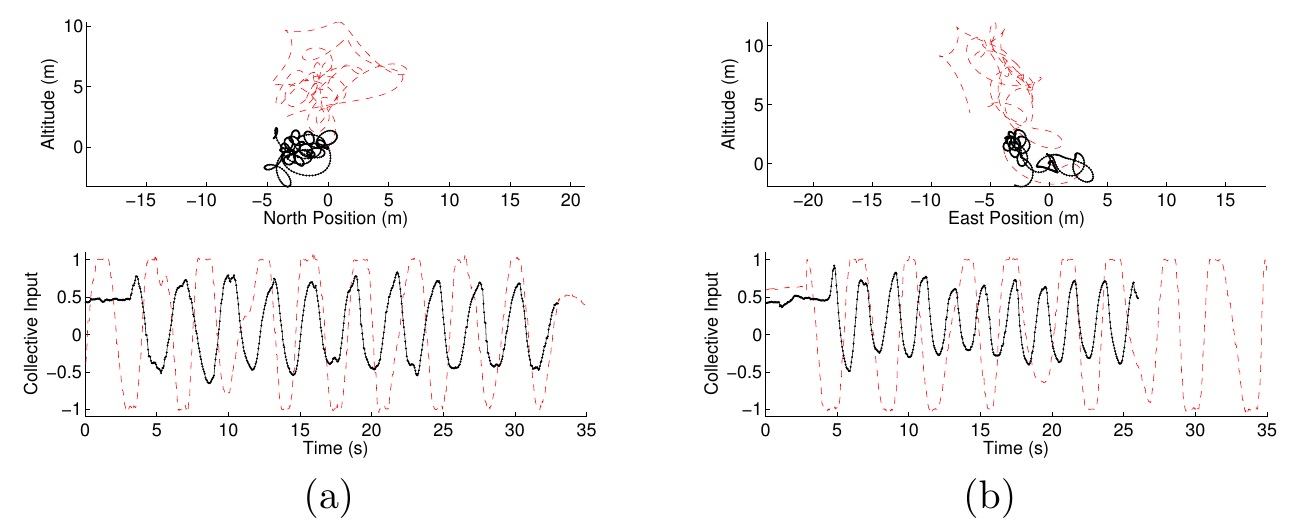
\includegraphics[width=1.0\textwidth]{figs/papers_ICAI2013_collectiveInput.png}
%%%%\caption{Collective input and resulting attitude of helicopter~\cite{2008_CNF_StanfordHeli_Coates}.} 
%%%%\label{fig:collective}				
%%%%\end{figure*}




For our experiments, we have procured a small-scale helicopter.  However, at this stage of our experiments, we have dealt only with simulations and use the dataset provided by the Stanford helicopter project (see Figure~\ref{fig:heli}).  Details on the hardware used in this project were taken from the website of the researchers, such as usage of a Synergy N9 airframe, an OS .91 engine, Futaba GY611 gyro, GV1 governor avionics with a nominal rotor speed of 1800 rpm and a ground-based vision system.  Each flight begins with the helicopter sitting on the ground for some time allowing for initialization.  Measured data include 9DOF accelerations, angular rates and magnetic field strength.  The interested reader is referred to~\cite{dataset_StanfordHelicopter} for more details.


%====================
\section{RESULTS}
%====================
%--------------------------------
\begin{figure}[t]
\centering	
\subfigure[Angular accelerations in $m/{sec}^2$ for $x$, $y$ and $z$ directions for states 1 and 2.]
{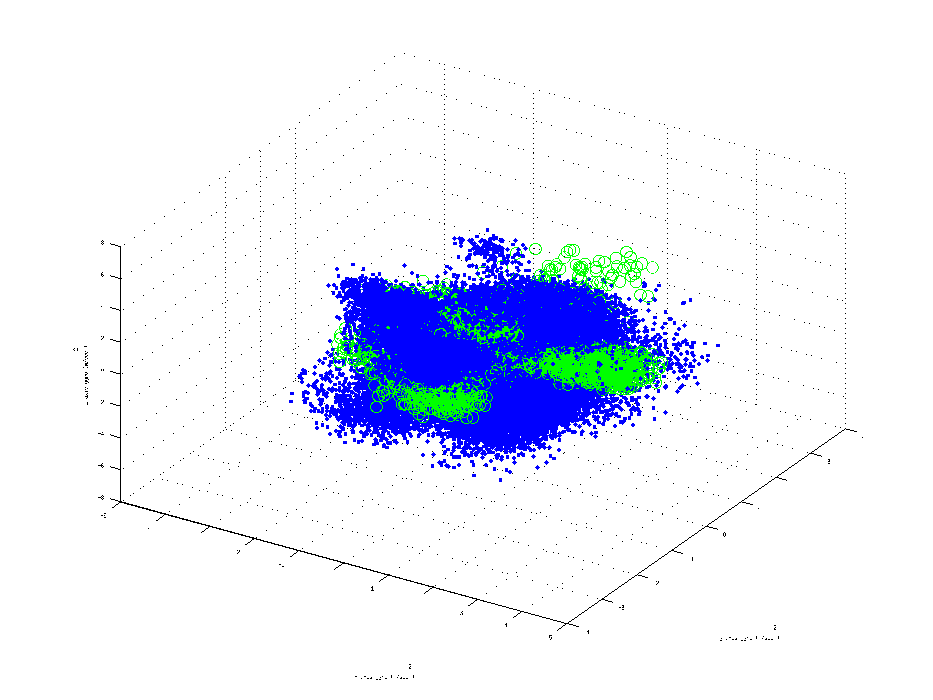
\includegraphics[width=0.45\textwidth]{figs/paper_10_ICAI2013_connectedClusters.pdf}\label{fig:connClusters}}
\subfigure[Pre-processing steps result in an increased measure of separability in the data.]{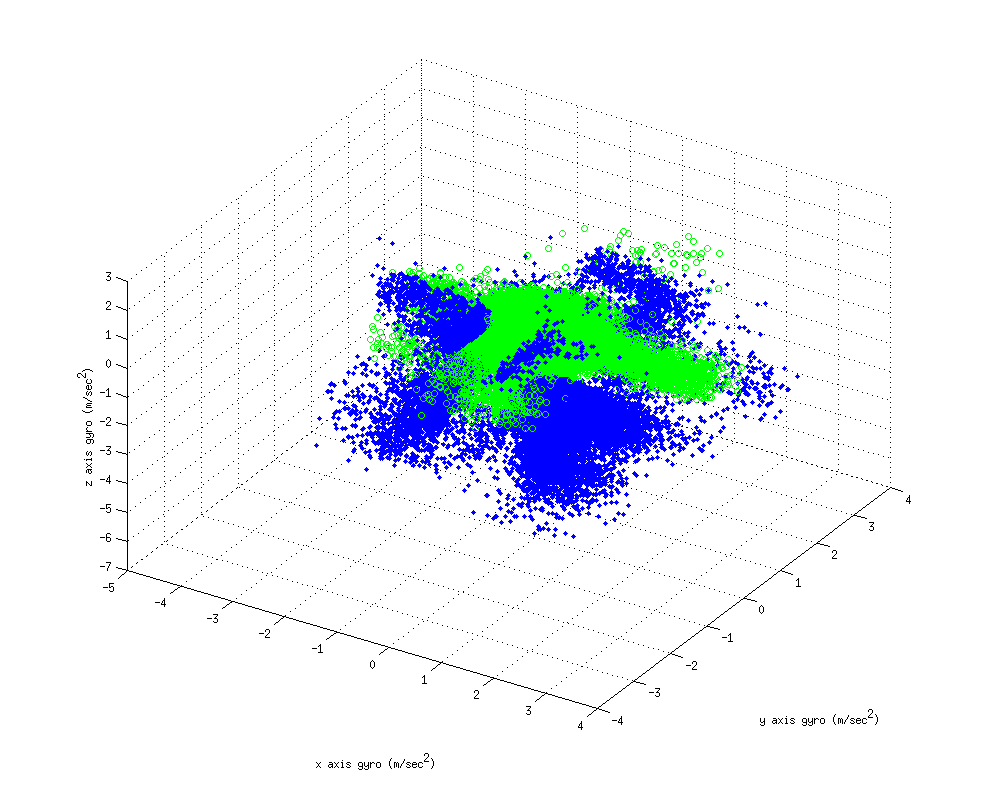
\includegraphics[width=0.45\textwidth]{figs/paper_10_ICAI2013_disconnectedClusters.png}\label{fig:disconnClusters}}
\caption{Data from the helicopter gyro.}			
\end{figure}


Our experiments and results focus on usage of RVQ to determine if the helicopter is in one of two dynamical states: (a) flying straight and level (state 1) and, (b) turning (state 2).  The reasoning behind this approach is that helicopter dynamics can be completely modeled over the entire flight envelope using a single non-linear model or a bank of linear models~\cite{2011_BOOK_Heli_Raptis}.  If a helicopter is to fly in autonomous mode, and if a bank of linear models is to be used, then a decision must be made in-flight as to which linear model to pick from the bank.  We use RVQ to assist in making this decision.

Given in Figure~\ref{fig:connClusters} is data from the helicopter gyro indicating angular accelerations in $m/{sec}^2$ for $x$, $y$ and $z$ directions.  Notice the overlap in the data for states 1 and 2.  After some pre-processing in which data around zero acceleration is discarded, we are able to generate some separation in the data as shown in Figure~\ref{fig:disconnClusters}.

At this point, a classifier, such as a Neural Network or a Support Vector Machine (SVM) could have been trained to classify the two states.  However, given the complex nature of the separating hyperplane that would be required, we decide to use a VQ based method.  The reason is that VQ naturally handles disconnected regions in the decision space.  Within the types of VQ that could have been used, we use RVQ due to its low memory requirements and linear computational complexity while at the same time giving performance comparable to exhaustive search VQ~\cite{1996_JNL_AdvancesRVQ_Barnes}.

While designing the stage-wise RVQ codebook, we check the reconstruction SNR of the input angular acceleration data-points and note that it is monotonically increasing as expected.  This is shown graphically in Figure~\ref{fig:RVQdecSNRdB} for every iteration.   For a stage-wise result, see Table~\ref{tbl: RVQSNRs}.

%--------------------------------
\begin{figure}[t]
\centering	
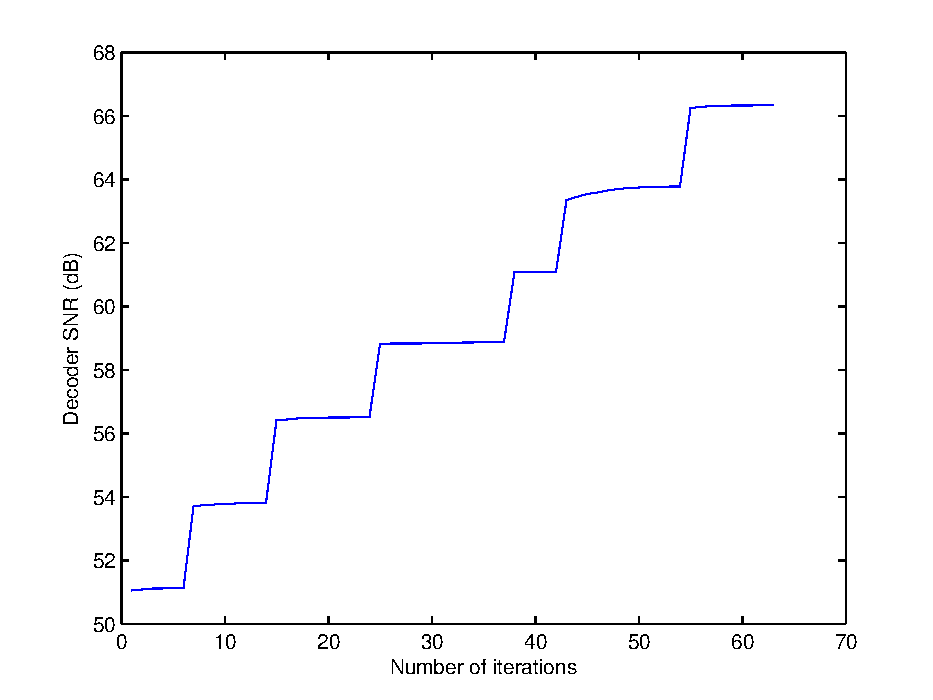
\includegraphics[width=0.45\textwidth]{figs/paper_10_ICAI2013_RVQdecoderSNRdB.pdf}
\caption{Monotonically increasing decode SNR for input datapoints while generating the RVQ codebook.  In this particular case, the RVQ codebook has $P=8$ stages with $M=4$ codevectors per stage.} 
\label{fig:RVQdecSNRdB}				
\end{figure}


%--------------------------------
\begin{figure}[t]
\centering	
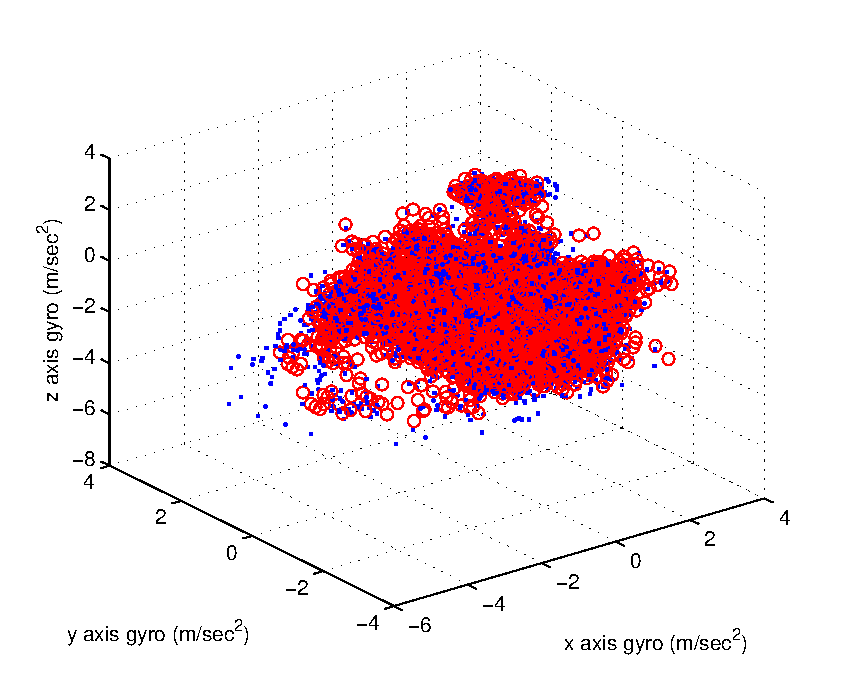
\includegraphics[width=0.45\textwidth]{figs/paper_10_ICAI2013_RVQreconstruction.pdf}
\caption{Reconstructing the input data points.  Notice that the actual data-points and reconstructed data-points are quite close to each other.} 
\label{fig:RVQrecon}				
\end{figure}

Indeed, Table~\ref{tbl:Results} shows that classification rate achieved is above 90\%.  Also shown in this table are some added statistics about the RVQ design process.

%--------------------------------
\begin{table}[h]
\center
\begin{tabular}{|c |c |}\hline
Metric & Value\\\hline
No of data points in $R^3$ & 17,893\\\hline
Time to train 8x4 RVQ codebook & 41.69 sec\\\hline
Classification rate & 92\% \\\hline
\end{tabular}
\caption{Final results.  Classification rate is high showing that RVQ can be used to determine which of two dynamical states the helicopter is in.  This can assist in picking the correct model for that particular state.  Picking the correct model is necessary for autonomous flight.}
\label{tbl:Results}
\end{table}

%--------------------------------
\begin{figure}[t]
\centering	
\subfigure[RVQ stage codevectors shown as circles within the data.  Here, we have used an 8x4 codebook, and so there are 32 stage-codevectors.  Using only these code-vectors, we have successfully reconstructed all data-points as shown in Figure~\ref{fig:RVQrecon} while maintaining high SNR as shown in Figure~\ref{fig:RVQdecSNRdB}.]
{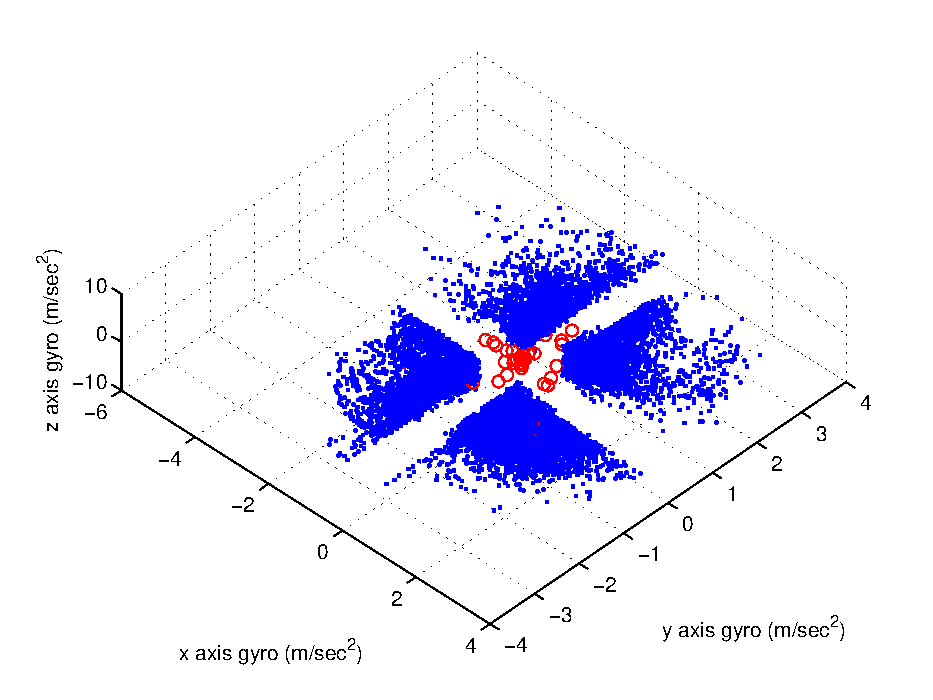
\includegraphics[width=0.43\textwidth]{figs/paper_10_ICAI2013_stageCodevectors.pdf}
\label{fig:rRVQstageCV}}
\subfigure[An example RVQ equivalent code-vector (direct sum centroid) shown as a circle.  Although most centroids lie within the data, some lie at the fringes as well.  This direct sum centroid lying at the fringe has been chosen for easier viewing.]{
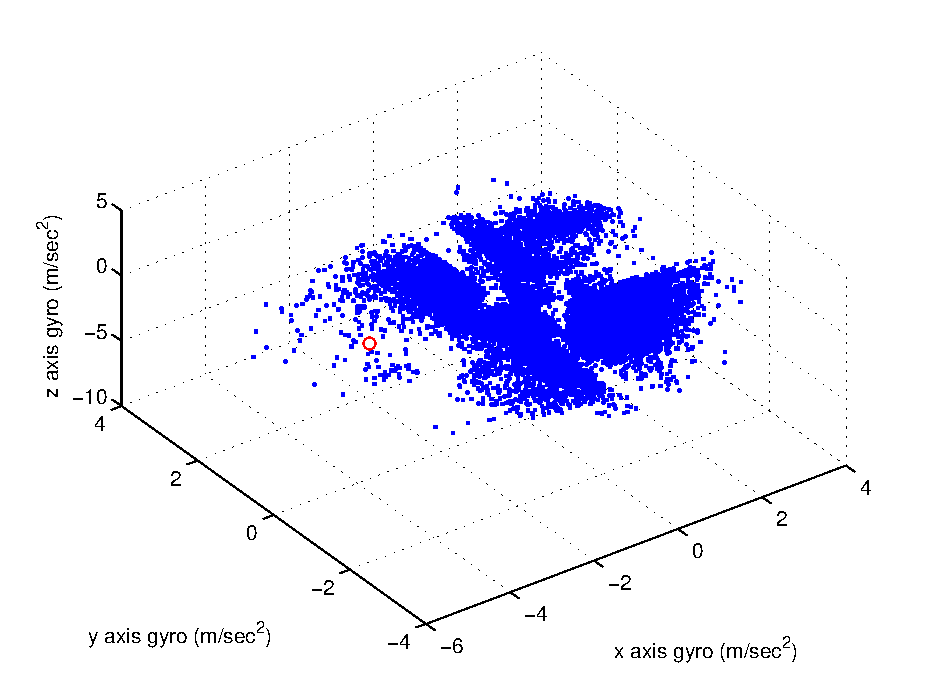
\includegraphics[width=0.43\textwidth]{figs/paper_10_ICAI2013_aDirectSumCentroid.pdf}\label{fig:rRVQdirectsumCV}}	 
\caption{RVQ code-vectors}		
\end{figure}


\begin{table}[t]
\center
\begin{tabular}{|c |c |}\hline
Stage & Reconstruction SNR (dB)\\\hline
1 & 51.13\\\hline
2 & 53.81\\\hline
3 & 56.61\\\hline
4 & 58.88\\\hline
5 & 61.08\\\hline
6 & 63.77\\\hline
7 & 66.34\\\hline
\end{tabular}\vspace{0.2in}
\caption{Reconstruction SNRs at the output of every stage for an 8x4 RVQ codebook.}
\label{tbl: RVQSNRs}
\end{table}

Reconstructions of the input data-points along with the actual data-points is shown in Figure~\ref{fig:RVQrecon} showing that the RVQ code-book correctly models the input data.  As a result, the hyperplanes in the decision space are expected to correctly classify the helicopter dynamical states.  

Shown in Figure~\ref{fig:rRVQstageCV} are the stage code-vectors of the 8x4 RVQ codebook used.  Notice that these stage code-vectors do not lie within the original data-points as it is summations of these code-vectors, 8 at a time, that will be used to generate all the data-points.  For illustration, a single equivalent code-vector, i.e, direct-sum codevector is shown in Figure~\ref{fig:rRVQdirectsumCV}.  As expected, this code-vector lies within the data.






 





%====================
\section{CONCLUSIONS}
%====================
In this paper, we have discussed initial work on using RVQ as a machine learning method for learning helicopter dynamics.  We have shown that helicopter states can be correctly classified using RVQ, a method whose run-time complexity and memory requirements are linear in the data.  In future work, we intend to extend this work in three directions, addition of more states, usage of data from our own small-scale helicopter, and learning complete non-linear helicopter dynamics using RVQ.  According to the best of our knowledge, the approach we have used is novel and it is hoped that RVQ will be brought to the attention of more researchers as a general purpose effective tool for conducting Machine Learning research.  Finally, we would like to thank Dr Christopher Barnes for allowing us to use his RVQ code for this research.

\bibliographystyle{IEEE}
\bibliography{MyCitations}

\end{document}
